Qt is a framework that streamlines the development of high-performance, visually appealing and feature-rich GUI applications. It offers support for multiple languages such as C++, Python, and JavaScript, allowing developers to choose their preferred language. Thanks to the documentation and the large user base, there is a lot of support material to reference \cite{qt}.

With the \hyperref[sub:qt_designer]{Qt Designer}, developers can create GUI designs effortlessly. Designs can be created via drag-and-drop, which accelerates designing in Qt. It also enables developers to visualize what their application will look like in real-time \cite{qt}.

The feature-rich and vast knowledge base, coupled with its user-friendly design, made it an easy choice to use in this project to develop the applications.


\section{Qt Designer}
\label{sub:qt_designer}

This is a tool from the Qt framework that allows designing and building a GUI via drag-and-drop. It uses the what-you-see-is-what-you-get approach, where how it looks in the designer will be the same in the real application \cite{qt}.

Figure \ref{fig:qt_designer} shows the Qt Designer application, which consists of a main window to which widgets can be dragged from the left sidebar to place them in the application. If a layout is selected for the widgets, Qt will automatically fit them according to the layout, so ensuring that the widgets are properly aligned. In applications, it is important to know the hierarchy of the widgets. Qt Designer makes this process easy to figure out, the object window (on the top right) shows the hierarchy tree of the widgets. Making a widget a child of another widget can be achieved by dragging it into the parent widget. 

Not only can the content and placement of the widgets be adjusted, but it is also possible to set several properties of these widgets within Qt Designer (on the bottom right). This helps to see the changes immediately without having to start the GUI application. This is especially useful when changing the style or the layout of certain widgets, as these changes are immediately reflected in the designer.

Qt Designer makes Qt an attractive choice for developers looking to create a GUI application. The real-time visualization makes creating a GUI easy and efficient, making it possible to try out different looks of the application, resulting in a modern-looking design with minimal effort.

\begin{figure}
    \centering
    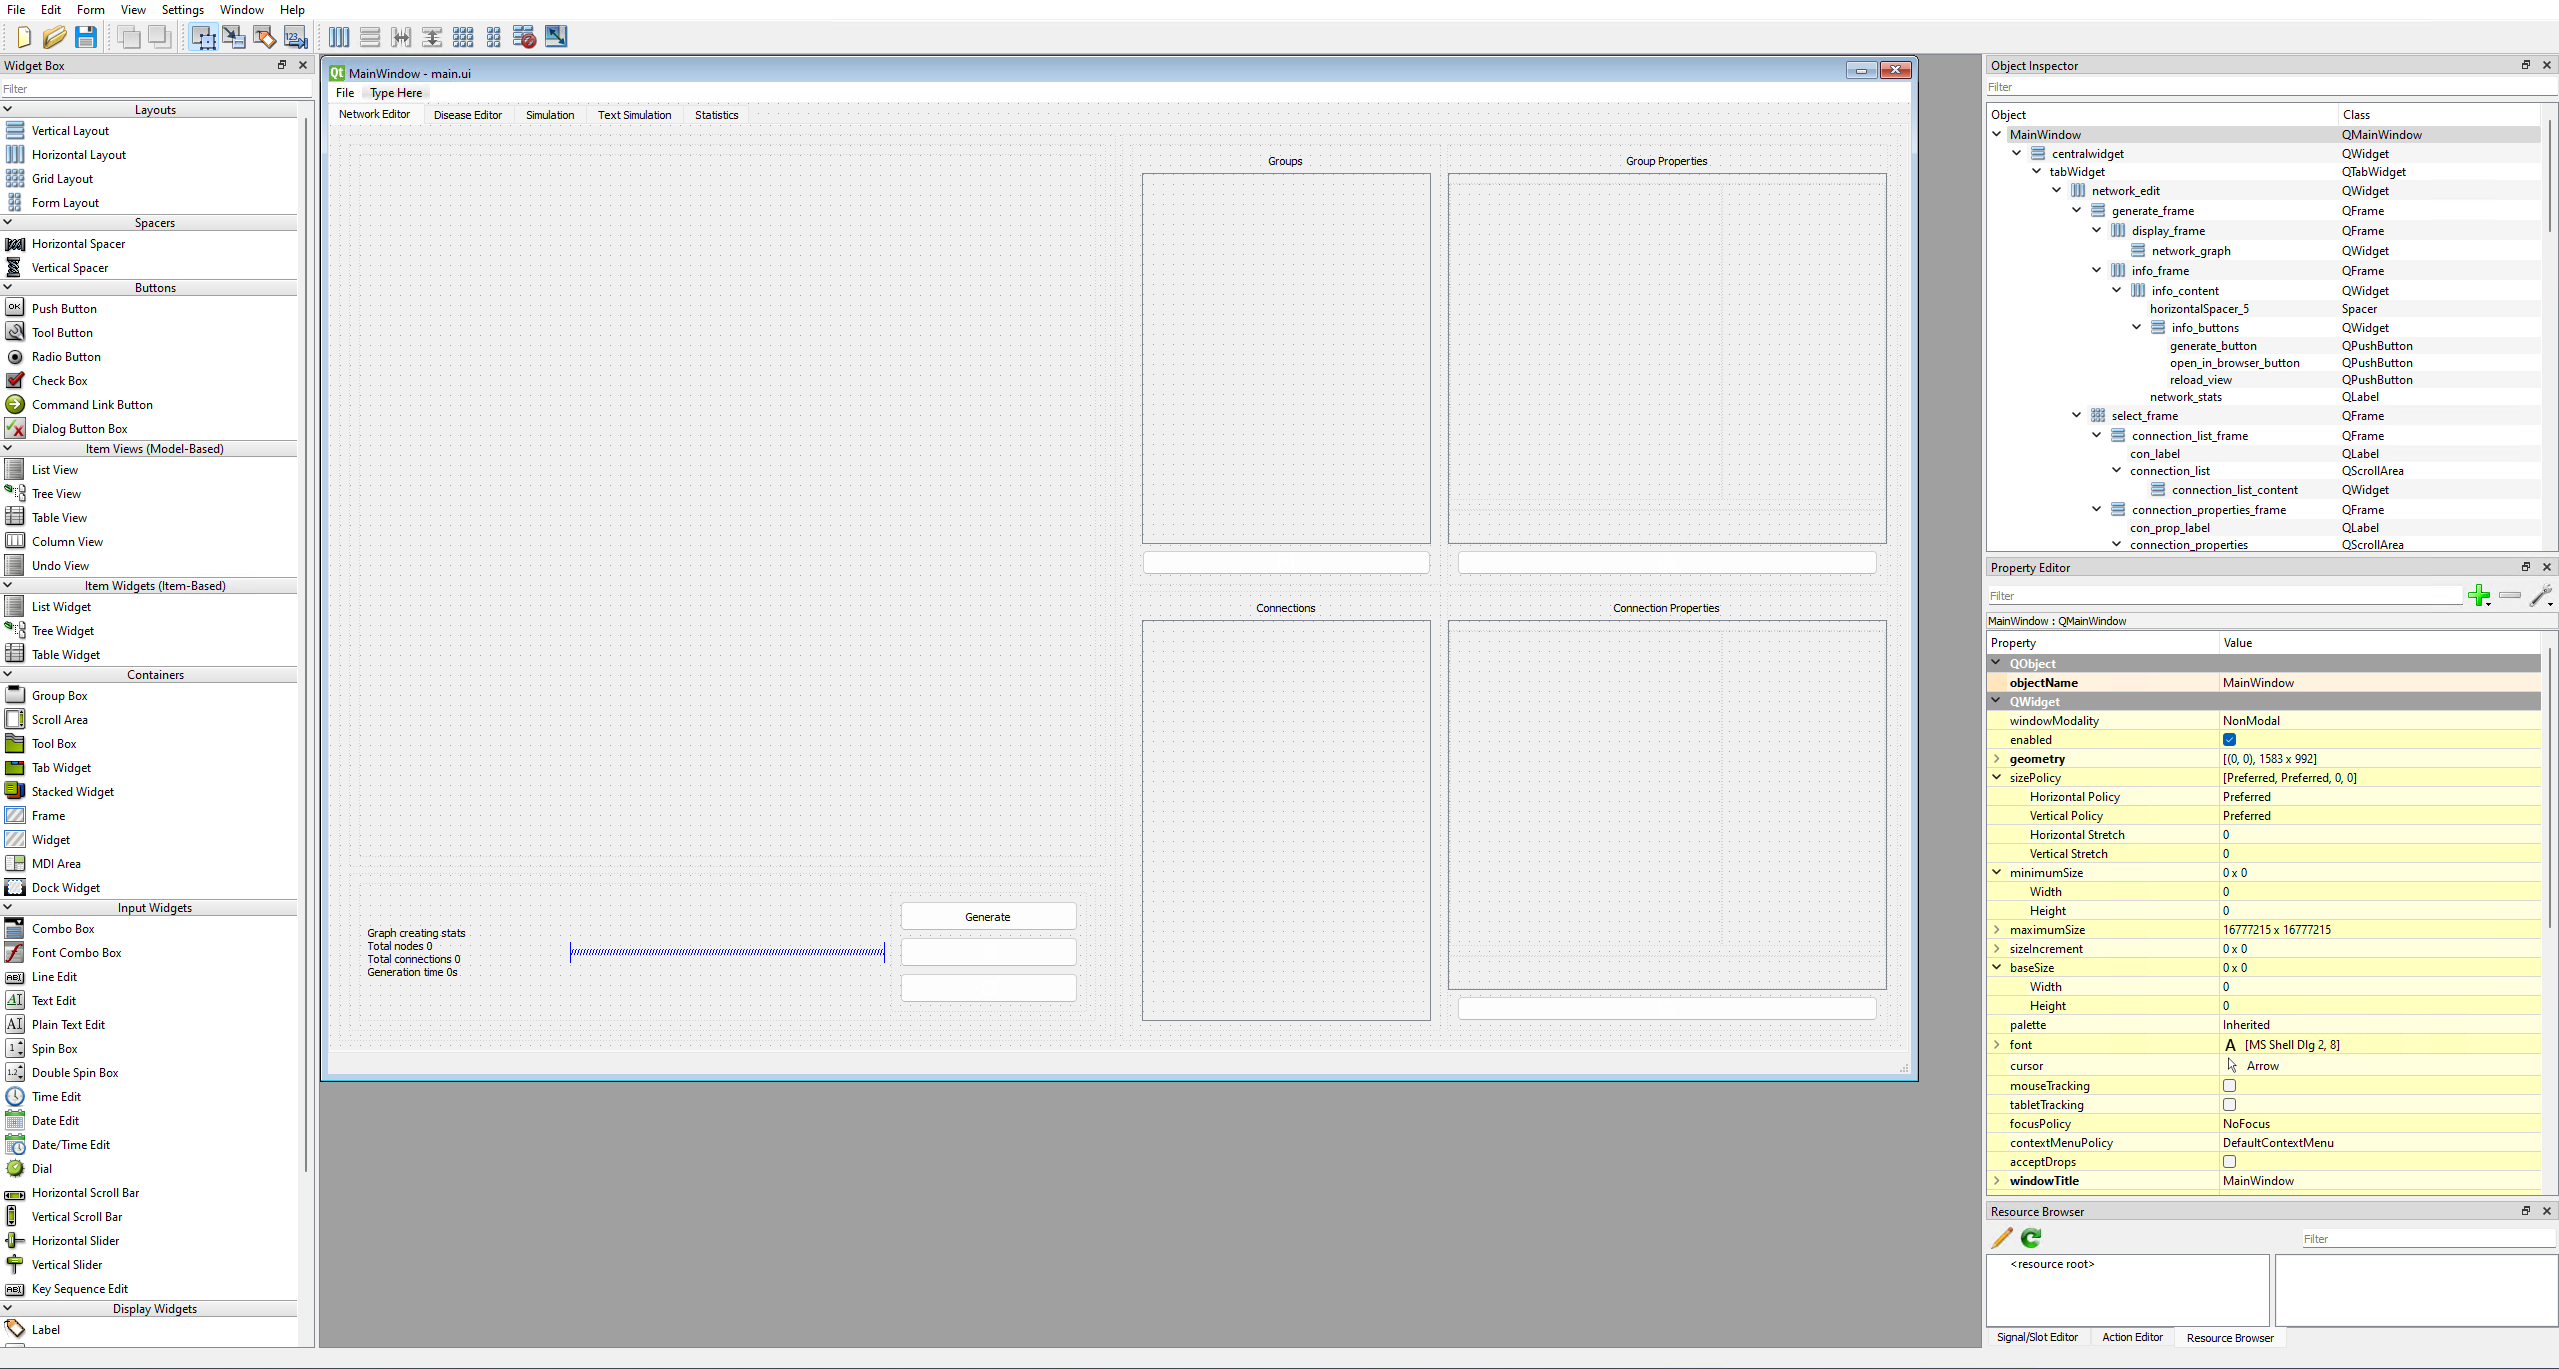
\includegraphics[width=0.8\linewidth]{images/qt_designer.png}
    \caption{Qt Designer}
    \label{fig:qt_designer}
\end{figure}

\section{PyQt}
\label{sub:pyqt}


Qt supports multiple programming languages to allow developers to choose their preferred language. This project was developed in Python, so PyQt was used. PyQt is a module that can be easily installed into the Python environment using pip. It contains all the add-ons that the C++ version of Qt also has. The add-ons can be used by importing the corresponding Python module. 

To develop an application in PyQt, the GUI can either be created using only the Python commands or with the help of the Qt Designer. The GUI created in the Qt Designer is saved in a \textit{.ui} file that can be loaded in the PyQt application \cite{pyqt}. Listing \ref{lst:pyqt_gui} shows how to load a \texttt{.ui} file into a simple application. 

Once a design is loaded into the application, it is easy to access the widgets that were created in the Qt Designer. To access and modify widgets created in the Qt Designer, they can be referenced using the ID associated with the widget in the designer. In Listing \ref{lst:pyqt_gui}, the widget created in the Qt Designer has the ID \textit{myLabel}. Depending on the type of widget, different functions are available, in this case the widget is a label, which contains the \textit{setText} function to change the text it displays. Other widgets, such as a frame widget, offer different functions. 

After a design is loaded, it is possible to add more widgets to it. For example, if buttons need to be created dynamically. This allows developers to create the default design of their application in the Qt Designer and dynamically change the content or arrangement of the widgets in the application. The ease of access to the objects created by the Qt Designer helps to improve the readability and simplicity of the application code.

\begin{lstlisting}[language=python, caption={Simple Qt GUI application}, label={lst:pyqt_gui}]
from PyQt5 import QtWidgets, uic
import sys
class GuiApplication(QtWidgets.QMainWindow):
    def __init__(self):
        super(GuiApplication, self).__init__()
        uic.loadUi('basic.ui', self)
        self.myLabel.setText('Changed text')
        self.show()

app = QtWidgets.QApplication(sys.argv)
window = GuiApplication()
app.exec_()
\end{lstlisting}

\section{Signals and Slots}
\label{sub:signals}

In GUI programming, it is often necessary to execute functions when, for example, a button is pressed. Other frameworks use callbacks to achieve this functionality; Qt uses the signals and slots mechanism. The signal is emitted by an object when its internal state changes. The slot is the function that will be executed once the corresponding signal is emitted. A signal can have multiple slots connected to it, which are executed one after the other. The signal-slot mechanism is independent of the GUI event loop and is executed immediately after a signal is emitted \cite{qt}.

Each signal has a \textit{.connect(Slot slot)} function that is used to connect the signal to a slot. For example, a button in Qt has three signals: \textit{clicked}, \textit{pressed}, and \textit{released}. In order to connect a function to the button, the following command has to be used: \textit{example\_button.clicked.connect(slot\_function)}. Now, when the button is clicked by the user in the GUI, the \textit{slot\_function} is executed \cite{pyqt}.

%TODO ein bsp aus dem code mit signal/slot aber halt nur für die buttons, weil ja danach erst die thread safety kommt
% TODO hopfully not shit
In this project, the signals and slots feature is mainly used to connect button presses and allow different objects to communicate with each other. The reason why signals should be used for objects to communicate with each other is explained in section \ref{sub:thread_communication}. Listing \ref{lst:signal_slot_example} contains a simple example from the project, that allows the user to start the network generation with a button press. To be able to start the generation process, the \textit{clicked} signal of the button \textit{generate\_button} is connected to the method \textit{start\_generating}. When the user presses the button, the slot is executed and therefore the generation process is started.
\begin{lstlisting}[language=python, caption={Signals and Slots example from the project.}, label={lst:signal_slot_example}]
class UiDisplayGroup(QObject):
    ...
    def connect_signals(self):
        self.generate_button.clicked.connect(self.start_generating)
        ...
    def start_generating(self):
        # Start the thread to generate the network.
\end{lstlisting}

\subsection{Thread communication}
\label{sub:thread_communication}

In general, it is bad practice to have a thread modify GUI widgets to ensure separation of concerns. If this thread were killed prematurely, it could result in an unexpected GUI state that could lead to errors. Or, if the main thread changed the structure of the GUI widgets before the thread could add the desired widgets, this would also lead to errors. To solve this issue, the signals and slots mechanism is ideal for this situation. Instead of letting a thread handle the widget creation, the thread just sends the widget data back to the main thread, which then adds or modifies the widgets. This way, the integrity of the GUI can be maintained because the main thread retains control over widget manipulation, ensuring consistent and expected behavior \cite{qt}.

% TODO hopfully not shit
An example of this approach is shown in listing \ref{lst:pyqt_thread_comm}. It demonstrates how the text simulation updates the label showing the current simulation speed. To achieve this functionality, three different classes were used:
\begin{description}
    \item[UiTextSimulationTab:] This runs in the main thread and changes the widgets.
    \item[SimulationWorker:] This class executes the simulation in a separate thread.
    \item[WorkerSignals:] This class only holds the signals that the threads can send.
\end{description}
First, an object for the class \textit{WorkerSignals} is created and stored as \textit{worker\_signals} in the \textit{UiTextSimulationTab}. The signals of this class are assigned to slots in the \textit{connect\_signals} method. Here, the \textit{update\_control\_label\_signal} is connected to the method \textit{update\_control\_labels}. When a user presses the buttons that changes the simulation speed, a signal is sent that executes the \textit{change\_speed} method that has been connected to the slot. This method changes the simulation speed according to the action sent as parameter. After changing the speed, this method sends the signal \textit{update\_control\_label\_signal}. This signal contains the current simulation speed. The simulation speed sent by the signal is received by \textit{update\_control\_labels}, which is executed in the main thread and can safely update the label containing the information. This way, only the main thread will change widgets.
\begin{lstlisting}[language=python, caption={Thread safety example}, label={lst:pyqt_thread_comm}]
class WorkerSignals(QObject):
    update_control_label_signal: pyqtSignal = pyqtSignal(float)
    ...
class SimulationWorker(QThread):
    ...
    def change_speed(self, action: str):
        # Changes the simulation speed according to the received action.
        self.signals.update_control_label_signal.emit(self.simulation_speed)
class UiTextSimulationTab:
    def __init__(self, parent: QtWidgets.QMainWindow):
        ... 
        self.worker_signals = WorkerSignals()
        ...
    def connect_signals(self):
        # Connecting the button Signals and other signals from the worker_signals
        self.worker_signals.update_control_label_signal.connect(self.update_control_labels)
    def update_control_labels(self, simulation_speed: float):
        # Updating the labels containing the simulation speed information.
\end{lstlisting}

\section{QSS}
% TODO hopfully not shit
Like HTML, Qt supports a style sheet to specify how widgets should look. QSS was inspired by CSS (Cascading Style Sheets) and is therefore very similar in terminology and syntax. A style sheet can be set for each widget either directly in the Qt Designer, in the code or in a separate file. If widgets are created dynamically and are not present in the Qt Designer, it is not possible for the Qt Designer to set the style for these widgets. In this case, either a style sheet file is needed, or the style must be set in the program itself \cite{qt}. The style sheet file has the advantage that it contains all the styles in one place rather than scattered throughout the program, which improves maintainability. The syntax for a style sheet is shown in listing \ref{lst:qss_example}. In this example, the padding and spacing for the \textit{QCheckBox} are changed. When a \textit{QCheckBox} is checked, it will display an image with the specified width and height.
\begin{lstlisting}[language=python, caption={QSS example}, label={lst:qss_example}]
QCheckBox{
    padding: 0px;
    spacing: 0px;
}
QCheckBox::indicator:checked {
    image: url(assets:selected.png);
    width: 24px;
    height: 24px;
}
\end{lstlisting}
% TODO hopfully not shit
To load a style sheet, it must first be loaded and then set as the style in the main application. PyQt5 has a method \textit{setStyleSheet} for every widget in Qt, which can be used to set individual styles for different widgets. It is also possible to set the style for the main application, which is used by all widgets in that application but is overridden by individual widget styles. Listing \ref{lst:load_qss}, shows how to set the style sheet as the main window style after successfully reading it \cite{pyqt}.
\begin{lstlisting}[language=python, caption={Loading of the QSS}, label={lst:load_qss}]
class UiNetworkEditor(QtWidgets.QMainWindow):
    ...
    def load_window(self):
        ...
        with open("qt/NetworkEdit/style_sheet.qss", mode="r", encoding="utf-8") as fp:
            self.stylesheet = fp.read()
        self.setStyleSheet(self.stylesheet)
\end{lstlisting}



\section{Abblication views}
\label{sub:thread_views}
The GUI application of the created app, contains five tabs/views, each with a different use:
\begin{description}
    \item[Network Editor] In this view, the user can create a network consisting of nodes and connections and view it in a 3D space.
    \item[Disease Editor] Allows to create the disease that are used for the simulation in the created network.
    \item[Simulation] The Simulation view embeds the webpage used for simulation. It displays the network and its state during the simulation, allowing the user to observe the behavior of the disease in the network.
    \item[Text Simulation] If the network is too big or a large number of simulation cycles are required, which makes using the visual simulation impractical, this text-based simulation can be used instead. It provides the same functionality for controlling the simulation and saving statistics as the visual simulation.
    \item[Statistics] This view embeds the webpage used to display the saved statistics. It can be used to view graphs for the various stats saved during simulations to help analyze the results.
\end{description}